\chapter{Conceptual Model}
\label{chap: Chapter 5}
In chapter 2, we discussed a brief history and introduced the three main types of recommender systems. The importance of this exercise was to review the literature and determine the inner workings of how recommender systems work. The corpus of papers revealed that nearly 55\% of papers employed the Content-Based Filtering (CBF) techniques of handling the content and the ranking system i.e., user profile building. This led to further exploration to find algorithms and techniques that will complement CBF. 

Chapter \ref{chap: Chapter 3} lays the groundwork and introduces various Machine Learning (ML) technologies. Primarily, chapter 3's literature was reviewed to shine a light on the machine learning field. However, it introduced complex interrelationships within its domain and the interaction of others. The complex interrelationships created the need to identify and approach employing various technologies covered in Chapters 2 and 3. 

In Chapter 4, the approach was not only set out; various stepping stones were discovered. The creation of the initial prototype was discussed in this chapter. Furthermore, common traps and concerns were identified i.e., feature extraction, selecting the number of topics, and the technology used to determine the similarity/recommend academic papers. 

In this chapter, The Recommendation Model, a conceptual model is developed to ease the intricacy surrounding the implementation of a NLP based recommender system. The recommendation model uses various algorithms and techniques derived from Chapters 2, 3, and 4. In 5.1, the model will be discussed from a birds-eye view. Later in the chapter, we will transition from an abstract level to a slightly more technical one. The above-mentioned technical overview will be covered in section 5.2.

\begin{figure}[htbp]
\centering
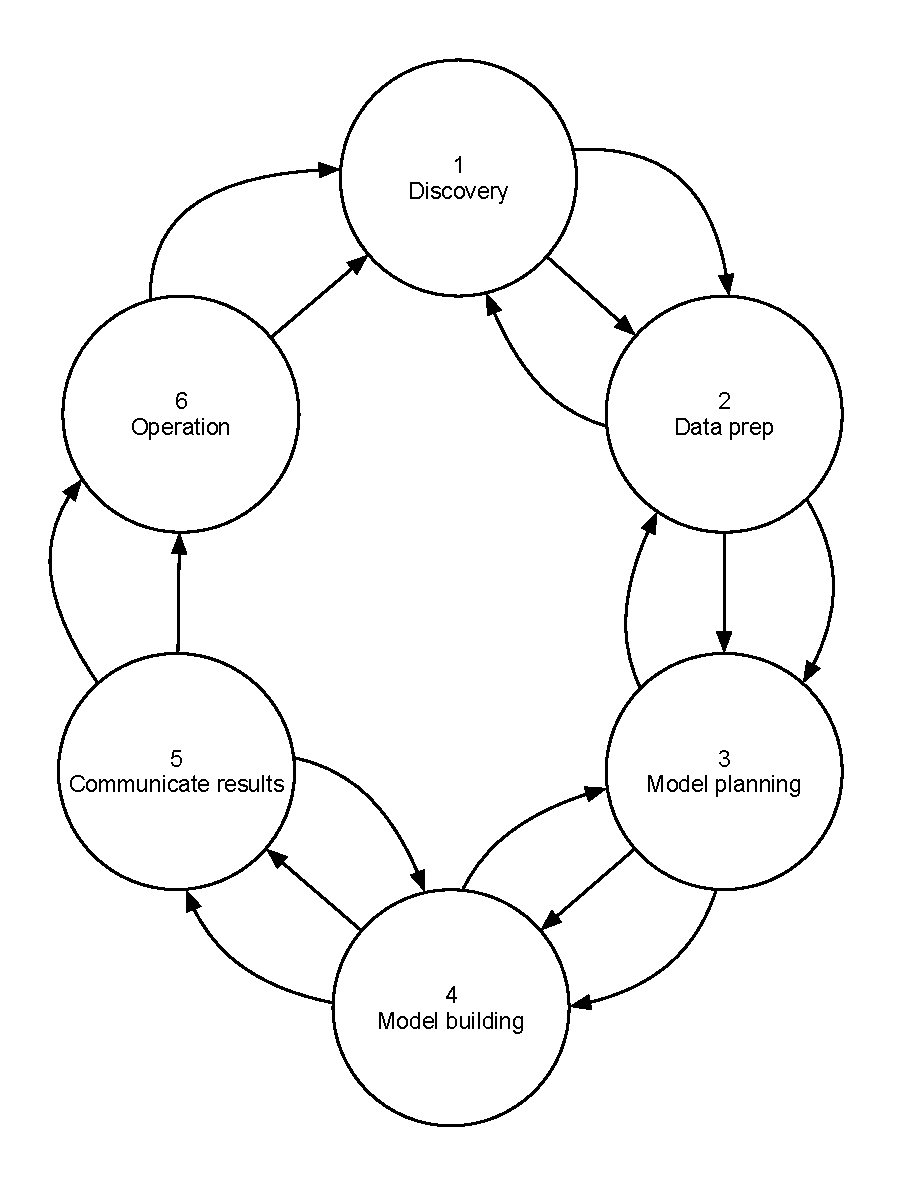
\includegraphics[width=8cm]{./figures/datalifecycle.eps}
\caption{Data Analytics lifecycle}
\label{fig:lifecycle}
\end{figure}

\section{Model Overview}
In recent years, research and development have been focused on creating a streamlined, widely acceptable Data Analytics Lifecycle. 

The goal of the Data Analytics Lifecycle was to have a structure in place that could aid teams and other researchers. Teams usually learn new things throughout their projects and often need to go back to the previous phase and refine the work based on new insights and information they have uncovered \cite{dietrich2015data}.
Each component of the data analytics lifecycle will briefly be discussed below \ref{fig:lifecycle}:
\begin{enumerate}
    \item Discovery - In this phase, discovering and gathering data is done. It is essential to best frame the data needs and obtains the correct data according to the requirements.
    \item Data Prep - The data must be correctly formatted to be used in a later phase. 
    \item Model Planning - This phase entails looking at various methods, techniques, and workflows that need to be employed to learn about the underlining relationships between the variables. 
    \item Model Building - Or also known as Analyze data, this phase focuses on analyzing the data and determining if the existing tools will suffice to get to the end goal.
    \item Communicate Results - In this phase, various visualization techniques will be considered and develop a summary to convey to the stakeholders.
    \item Operationalize - Or also commonly known as Making Decisions. This phase focused on delivering reports, code and other technical documents
\end{enumerate}

\begin{table}[htbp]
\centering
\begin{tabular}{|l|c|c|}
\hline
\textbf{Known terminology} & \textbf{Study terms} & \textbf{Domain of techniques} \\ \hline
Discovery & Past papers & Dataset\\ \hline
Data prep & Preprocessing & Machine learning - Chapter \ref{ssec:prep}\\ \hline
Model planning & Learning & ML + IR - Chapter \ref{chap: Chapter 3} \\ \hline
Model building & Human intervention & Prototype - Chapter \ref{ssec:prot} \\ \hline
Communicate results & Represent in data frame & Discussion - Chapter \ref{chap: Chapter 7}\\ \hline
Operation & Enable decision makers & Evaluation - Chapter \ref{ssec:eval} \\ \hline
\end{tabular}
\caption{Mapping between terminologies used in study}
\label{tab:mapping}
\end{table}

\begin{figure}[htbp]
\centering
\includegraphics[width=8cm]{./figures/overview3.eps}
\caption{The Recommendation Model overview}
\label{fig:Modeloverview}
\end{figure}

Above being said, the researcher had felt the need to provide a mapping between the terminology used in the research domain and this study. As seen in figure \ref{tab:mapping}, it should be known that when the researcher is using terminology like past papers, preprocessing and learning it holds the exact contents of its corresponding terms used in research. The column on the right in figure \ref{tab:mapping}, can be translated to be the domain and or section within this study which addressed each phase of this model.


This section of the chapter covers the model overview as seen in figure \ref{fig:Modeloverview}. The model is categorised into three components: (1) Past papers, (2) learning, and (3) Processing.

Past Papers can be identified as the core of the model. This is made up of past or historical papers. This will then flow into the Learning component, which is a fundamental stepping stone in defining what needs to be done. In the Processing component, the model looks at the defining functions in Learning and further refines them. Learning and the Processing component will be discussed further in this chapter.

\section{Learning}
The Learning component is created by closely analysing past papers. The goal was to understand better the characteristics which made up the Learning component. The conceptual model is constructed in such a way that it is not only Information Security domain-specific. This being said, the characteristics of the Learning were identified and guided by literature. The characteristics of the Learning are:
\begin{enumerate}
    \item Populating stopword list
    \item Stemming
    \item Topics of the model
    \item Measuring the similarities
\end{enumerate}

\begin{figure}[htbp]
\centering
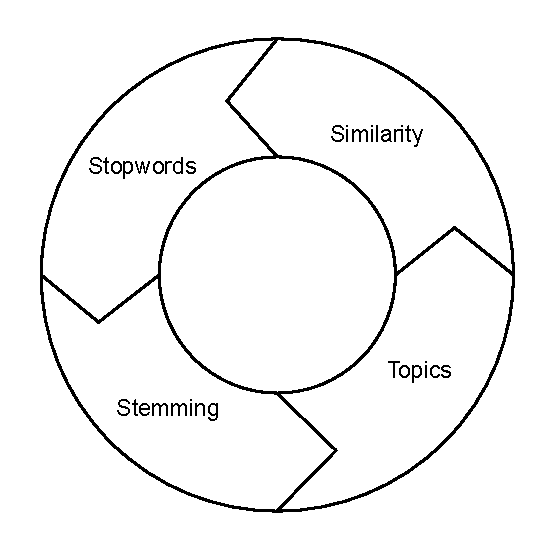
\includegraphics[width=8cm]{./figures/learning.eps}
\caption{Learning Component}
\label{fig:core}
\end{figure}
The flow of the Learning is using the stopword list, then stemming those words,  stemming leads into topics that will be generated, and the similarity of these topics will be measured. As seen in figure \ref{fig:core}, the Learning component's flow leads one character into another. The reason for this is that the Learning component is a continuous process. Each of these characteristics is described in the following sections.

\subsection{Populating stopword list}
The stopword list was primarily made up of NLTK's stopword list. The goal of this choice was to employ a stopword list that had a comprehensive list of words. NTLK is one of the widely used NLP libraries.
Furthermore, after close consideration, additional words were included in the stopword list as time passed. These words were primarily domain-specific such as: (1) Information, (2) Technology, and (3) Security.

The goal of the inclusion was to retrieve second or third-tier topics from the text. The textual outputs of each component of the Learning component were analyzed, and words that did not bring any value or words which was primary domain-specific were omitted.

The process of including words and excluding others was a manual and iterative process. The resulting words were best suitable for the Information Security domain and were used as the stopword list.

\subsection{Why Stemming?} \label{ssec:stemming}
Stemming was employed for the sheer simplicity and thorough work it has done. To recap, stemming is removing the suffix of the word to return it to its root form. 
The Porter stemmer is appropriate to IR research work involving stemming where the experiments need to be exactly repeatable. This being said, after consulting the dataset, it was identified that the domain in which this research position itself did not need to have a custom-made stemming solution.

After close consideration, the researcher, along with evidence, used Porter Stemmer from the NLTK library.

\subsection{Topics of the model}
The Information Technology domain is such a rich field with regards to topics and subtopics. It needed to be scoped down to provide better topics for the algorithm to use. For example, Information, Technology and Security would be excluded. As seen in \ref{fig:core}, all of the components feed into one another. In this case, specific topics names were appended in the stopword list. 
The result of the methodology mentioned above was smaller topics. These were second and third-tier topics, such as hacking and Man-in-the-middle attacks, respectively.
A few of the lower-tier topics fused make up the second tiers topic. This also holds for second-tier and first-tier topics.

\subsection{Measuring the similarities}
The vast amount of topics made it challenging to group similarities of papers. The topics were too dense from a dimensionality perspective. For the scope of this research, similarity algorithms reduced dimensionality. In addition to the dimension reduction, the unsupervised learning approach made it viable to use an algorithm to cluster similar topics. This would have a direct impact on measuring the similarities in the academic papers.

\subsection{Learning component summary}
There are four components of the conceptual model. They were discovered by reviewing literature and building a proof of concept. The first component on the list, stopword removal, is fundamental in getting the text ready for further analysis. The stopword list is compiled by using the standard NLTK stopword list and adding a few first tier Information Security topics, to reduce scope. 

The second component, stemming, removes the suffix of certain words to take them to their root form. The third component, topics, the corpus exists of various tiers of topics. a Collection of specific tier topics would form a topic in a higher tier. The similarity between these topics would then be calculated to reduce dimensionality and cluster most similar topics together.
\section{Processing}
In this section, the next phase of the conceptual model will be discussed. The Academic paper processing phase is executed when a new and unseen academic paper is submitted. Just like the Learning component, this phase also has four components. It is merely an extension of the components found in the Learning component. 

In the first step, the fundamental stepping stone, the removal of stopwords, will be actioned. The new document will have its stopwords removed to simplify and get the text ready for further analysis. Step two includes taking the text that was cleaned and stemming it. This will remove the suffix and return the words to their root form. Step three's goal is to get the related topics in the text. The last step, step 4, will focus on using the topic output and determining the topics' similarities. These four component is best described in the figure \ref{fig:processing}, and a brief description of each component is in the following sub-sections.
\begin{figure}[htbp]
\centering
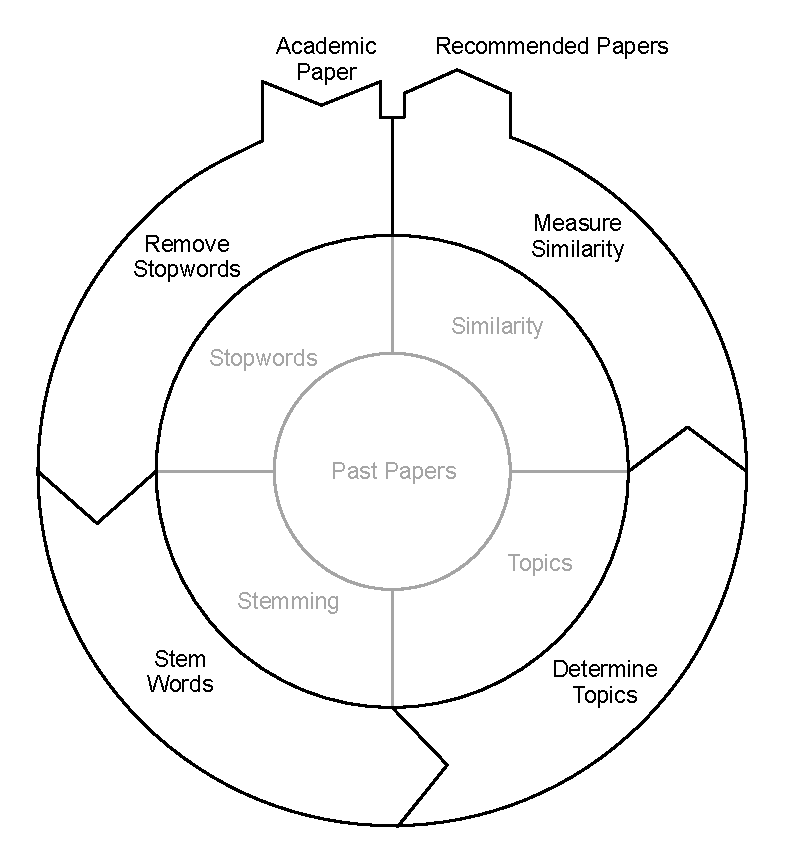
\includegraphics[width=8cm]{./figures/processing1.eps}
\caption{Processing phase of the model}
\label{fig:processing}
\end{figure}
\subsection{Removing the stopwords}
The stopwords are removed from the collection of documents. The goal was to remove the words that do not bring any meaning to the sentences. Terms such as 'specified' , 'specify', 'specifying', furthermore, The stopword list also included words such as 'information', 'security' and 'technology'.
\subsection{Stemming of the words}
After the stopwords were removed, the tokenized dataset was then stemmed. For example, the words mentioned above 'specified' , 'specify', 'specifying' can be stemmed and will look like the following: ' specif', 'specif', 'specif'. As explained in the Learning component section of this chapter, stemming is removing the word's suffix to return the term in its root form. The stemmed words are then used to determine topics.
\subsection{Determining the topics} \label{ssec:topic}
This component comprises of determining the topics of the dataset. This is done after the stopwords were removed and after the text was stemmed. A topic modeling technique will then be applied to the dataset after it is transformed. The soft clustered topics would look something like this, '0.040*"data" + 0.033*"file" + 0.024*"encrypt" + 0.021*"cloud".
A similarity ratio of the terms is calculated, and the most similar terms were clustered together, forming topics. 
\subsection{Measuring the similarities}
At this point of the conceptual model, the stemmed words that do not contain any stopwords have been pushed through the topic modeling technique. The product of the previous three components was a collection of topics that represents the dataset. The collection of topics of the dataset and the topics of the test set were measured in terms of similarity. The lower the score, the more similar the two papers are with one another.
\subsection{Processing phase summary}
In this section, we discussed the Academic Paper Processing phase. This phase is executed when a new document is submitted. The dataset would already remove the stopwords, stemmed, and determine the topics. Once a new document is submitted, it will go through the same process. The only difference here is that the similarity of the two datasets will then be measured. The topics with the lowest score will be most similar.
\section{Conclusion}
The conceptual model presented in this chapter is a template for finding similar academic papers. The use case for this research is focused on Information Security academic papers. However, it can be used to find any academic papers across disciplines. The conceptual model is built on a collection of academic papers or datasets. Various Learning components were identified while surveying the field. The Learning components were broken down into four distinct components: (1) stopword, (2) stemming, (3) topics, and (4) similarity. 

After the Learning component was built through experimentation, it was ready and waiting for new academic papers to do the testing. The Academic Paper Processing phase could then begin. Just like the Learning components, the Academic Paper Processing phase also has four components. 

Firstly, the dataset was cleaned from all the stopwords. Special consideration was made for the 1st tier topics like 'Information' and 'Security', and those were also included in the stopword list. 

Secondly, once the stopwords have been removed, next, would be to stem the remaining data. Stemming commonly includes omitting the suffix of a word. This is done to return the word to its root form. 

Thirdly, topics were determined by using a topic modeling technique. The technique helped soft cluster all the similar terms together, which formed topics. These topics consist of the 'training set' corpora. Once a 'test set' document appears, it will run through the same components.

Once we have the 'training set' and 'test set' ready, the last component measures the similarity between the two sets. The new, unseen 'test set' document would then be hard clustered to the most similar set of topics. The next chapter, Model implementation, and refinement, describes how the conceptual model is implemented and refined.